% СПО ЛКС - TCP/IP
% Пынькин Д.А. (с) 2011
\documentclass[ignorenonframetext, hyperref={pdftex, unicode}]{beamer}
\usepackage{beamerthemesplit}

\usetheme{Pittsburgh}
\usecolortheme{dolphin}

\usepackage[russian]{babel}
\usepackage[utf8]{inputenc}
\usepackage[T1]{fontenc}
\usepackage{ulem}
%\usepackage{html}

\usepackage{verbatim}

\usepackage{tikz}
\usetikzlibrary{positioning,arrows}

\title[СПОЛКС (http://goo.gl/32cTB)]{Системое программное обеспечение локальных компьютерных сетей}
\author{Денис Пынькин}
\date{2011 -- 2012}
%\institution[БГУИР]{Белорусский государственный университет информатики и радиоэлектроники}
%\logo{
\includegraphics[width=1cm]{logo-kafEVM.png}}


\subtitle{Стек протоколов TCP/IP}

\begin{document}

\mode<all>{\begin{frame}
\titlepage
\begin{center}
e-mail: denis.pynkin@bsuir.by\\
\end{center}
\begin{center}
{\bfseries http://goo.gl/32cTB}

{\tiny СЧАСТЬЕ ДЛЯ ВСЕХ, ДАРОМ, И ПУСТЬ НИКТО НЕ УЙДЕТ ОБИЖЕННЫЙ!\\
(c)Стругацкие, Пикник на обочине}
\end{center}
\end{frame}
}

\tikzstyle{format} = [rounded rectangle,
                      thick,
                      minimum size=1cm,
                      draw=red!50!black!50,
                      top color=white,
                      bottom color=red!50!black!20,
                      font=\itshape,
                      drop shadow]
%
% Далее начинается сама презентация
%
\section{TCP/IP}

\begin{frame}{Даты}
	\begin{block}{1975}
	Первый тест между двумя системами
	\end{block}
	\pause
	\begin{block}{1977}
	Тестовая сеть между тремя системами США, Великобритании и Норвегии
	\end{block}
	\pause
	\begin{block}{1978-1983}
	Тестируется 4 версии стека TCP/IP. И только в 3-й происходит разделение на протоколы TCP и IP.
	\end{block}
	\pause
	\begin{block}{Март 1982}
	US DoD объявляет стек TCP/IP стандартом для военных сетей.
	\end{block}
	\pause
	\begin{block}{01 января,  1983}
	День рождения Интернет -- именно в этот день Arpanet официально переключилась с NCP на TCP/IP 
	\end{block}
\end{frame}


\begin{frame}{Стек TCP/IP}
	\begin{center}
		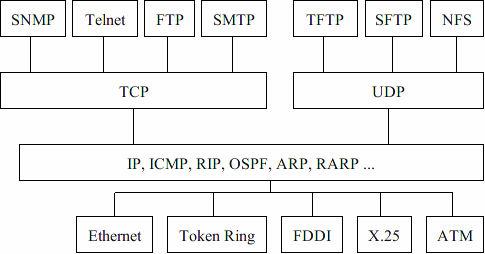
\includegraphics[width=1\textwidth]{03-TCP_IP.png}
	\end{center}
\end{frame}

\mode<all>{\begin{frame}{}
\Huge
\begin{center}
	Спасибо за внимание!
	\bigskip
	Вопросы?
\end{center}
\normalsize
\end{frame}
}

\end{document}
%Конец файла
